\documentclass{ML}
\usepackage{hyperref}
% 姓名,学号
\infoauthor{朱明彦}{1160300314}

% 课程类型,实验名称
\infoexp{课程类型}{实验二}

\infoschool{计算机学院}{杨东华、王金宝}

\begin{document}
\maketitle

\tableofcontents
\newpage

\begin{center}
    \textbf{\zihao{3} 实验二 \  聚类与分类}
\end{center}

\section{实验目的}
掌握对数据使用聚类分析和分类分析,并理解其在大数据环境下的实现方式。
\section{实验环境}
\begin{itemize}
    \item Ubuntu 16.04
    \item Hadoop 2.7.1
\end{itemize}
\section{实验过程及结果}
% 对于实验内容3.1-3.4,请结合您的程序描述实验中各个数据预处理步骤的详细操作,并说明每一步的输入和输出,包括输入输出数据的内容、格式等信息。
\subsection{聚类分析}
\subsubsection{KMeans聚类分析}
\paragraph{主要思想}
利用两类Mapper和Reducer,其中第一对Mapper-Reducer主要用于中心点的选择,即初始化等工作;第二对Mapper-Reducer主要用于中心点的选择,即初始化等工作;第二对Mapper-Reducer主要用作迭代过程。

对于K值的选择,参考CMU在2014年春季的10-605\cite{kmeans-mr-k},使用8或者12作为聚类中心数。
\paragraph{第一类Mapper}
\begin{itemize}
    \item 输入:原始数据
    \item 输出:\texttt{(1, 原始数据中的一条)},共K个。
    \item 随机选择K个元素作为初始化的聚簇中心点,利用\texttt{run}函数实现。
\end{itemize}
\textbf{由于此处仅仅需要K个元素作为初始化的聚簇中心点,所以只能使用1个第一类Mapper处理原始数据。}
\paragraph{第一类Reducer}
\begin{itemize}
    \item 输入:\texttt{(1, [$c_0, c_1, \dots, c_{k-1}$])},其中$c_i, i \in \{0, 1, k-1\}$为原始数据中的一条。
    \item 输出:\texttt{($i$, $c_i$ + \texttt{$\backslash$t} + '-1')},其中$i$为聚簇编号,$\backslash$t为制表符,加法为定义在String上的加法,即字符串的连接。
\end{itemize}
对于第一类Reducer而言,其输入的元组Key均为1,所以仅有1个第一类Reducer。

\paragraph{第二类Mapper}
\begin{itemize}
    \item 输入:原始数据
    \item 输出:\texttt{(clusterCenterID, $v;minDis$)},其中Key为\texttt{clusterCenterID},即该元组距离最近的聚类中心的编号;Value为$v;minDis$,其中$v$为该条原始数据,$minDis$为该原始数据与最近的聚类中心的欧式距离,二者以英文分号“;”分割。
\end{itemize}

\paragraph{第二类Reducer}
\begin{itemize}
    \item 输入:\texttt{(clusterCenterID, [$v_0;minDis_0$, $v_1;minDis_1$, $\dots$])}
    \item 输出:\texttt{(clusterCenterID, $new_c$ + \texttt{$\backslash$t} + disSum)},其中$new_c$为属于该聚簇的计算出的新的聚类中心,\texttt{disSum}为所有属于该聚簇的元素到该中心的距离和,用于判断Kmeans迭代收敛。
\end{itemize}

\textbf{最终的Kmeans实现步骤如下,相关结果如图\ref{fig:kmeans}所示。}
\begin{enumerate}
    \item 使用1个第一类Mapper随机取K个聚类中心,利用Reducer将结果存入HDFS。
    \item 读入上一轮(或者随机取的K个元素)中心点,并利用Configuration保存中心点。
    \item 利用第二类Mapper计算每个元素所属的聚簇。
    \item 利用第二类Reducer重新计算聚簇中心。
    \item 如果收敛,算法结束;否则重新返回第2步。
\end{enumerate}
\begin{figure}[hbt]
    \centering
    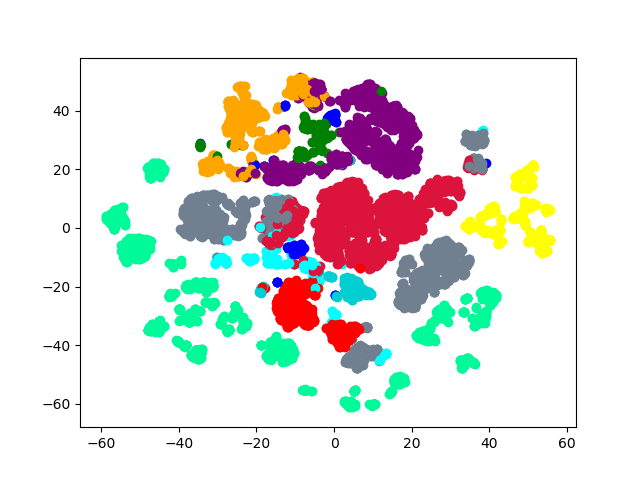
\includegraphics[width=0.8\linewidth]{media/cluster_1.png}
    \caption{KMeans聚类结果}\label{fig:kmeans}
\end{figure}
\subsubsection{GMM(混合高斯模型)聚类分析}
\paragraph{原理}
参考\cite{ml-book}图9.6,主要使用了两类Mapper和Reducer,其中第一类Mapper-Reducer负责读取Kmeans的结果作为初始化的均值并初始化协方差阵;第二类Mapper-Reducer利用EM算法更新每个高斯分量的均值、协方差和混合系数。

\paragraph{第一类Mapper}
\begin{itemize}
    \item 输入:KMeans聚类中心
    \item 输出:\texttt{(1, value)},其中Key为1,保证所有的值都在同一个Reducer中处理,\texttt{value}为聚类中心。
\end{itemize}

\paragraph{第一类Reducer}
\begin{itemize}
    \item 输入:\texttt{(1, [value$_0$, $\dots$, value$_{k-1}$])}
    \item 输出:\texttt{(i, $\pi_i, \mu_i, \sigma_i$)},其中Key为i,即第i个高斯分量;$\pi_i, \mu_i, \sigma_i$分别为第i个高斯分量的混合系数、均值和协方差阵,均以字符串进行存储。
\end{itemize}

\paragraph{第二类Mapper} 负责处理EM算法中的E步。
\begin{itemize}
    \item 输入:原始数据
    \item 输出:\texttt{(i, $\gamma_{ij}$)},KEY为高斯分量的标号i,$\gamma_{ij}$给出样本$\mathbf{x_j}$由第i个高斯分量生成的后验概率\cite{ml-book}。
\end{itemize}

\paragraph{第二类Reducer} 负责处理EM算法中的M步。
\begin{itemize}
    \item 输入:\texttt{(i, [$\gamma_{i0}$, $\gamma_{i1}$, $\dots$, $\gamma_{iN}$])},其中$N$为样本数量。
    \item 输出:\texttt{(i, $\pi'_i, \mu'_i, \sigma'_i$)},其中Key为i,即第i个高斯分量;$\pi'_i, \mu'_i, \sigma'_i$分别为第i个高斯分量新的混合系数、均值和协方差阵。
\end{itemize}

最终GMM实现的步骤如下,实验结果如图\ref{fig:gmm}所示,迭代固定轮数为10轮(由于计算的复杂度过高):
\begin{enumerate}
    \item 读入KMeans结果,利用第一对Mapper和Reducer初始化K个高斯分量的混合系数、均值和协方差阵。
    \item 利用第二类Mapper实现EM算法的E步,即计算每个样本由各个高斯分量生成的后验概率。
    \item 利用第二类Reducer实现EM算法的M步,即更新每个高斯分量的混合系数、均值和协方差阵。
\end{enumerate}

\begin{figure}[hbt]
    \centering
    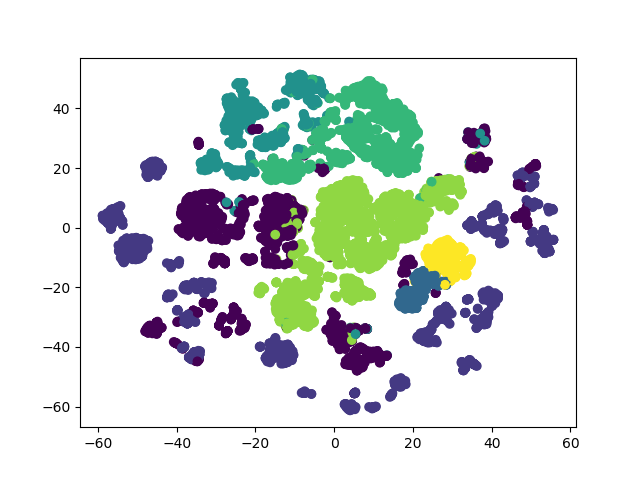
\includegraphics[width=0.8\linewidth]{media/GMM.png}    
    \caption{GMM聚类结果}\label{fig:gmm}
\end{figure}
\subsection{分类分析}
\subsubsection{朴素贝叶斯}
\paragraph{原理}
由于使用的数据每一维特征都是连续型的数据,所以其处理与离散型的朴素贝叶斯处理有所不同。\textbf{因此,假设数据的每一维都符合高斯分布,而高斯分布的均值和方差均通过训练数据中的均值和方差来代替。}
数据第$i$维取值为$x_i$的类条件概率为:
$$
    P(X_i = x_i | Y = y_j) = \dfrac{1}{\sqrt{2\pi\sigma_{ij}^2}}e^{-\frac{(x_i - \mu_{ij})^2}{2\sigma_{ij}^2}}
$$
其中$y_j$为第$j$类,$\sigma_{ij}, \mu_{ij}$分别为第$j$类第$i$维样本数据的均值和方差。具体实现时,利用了两类不同的Mapper和Reducer,其中第一对Mapper和Reducer主要用来计算训练数据中类别的先验;而第二对Mapper和Reducer用于处理计算后验并确定每一个样本所属的类别。

\paragraph{第一类Mapper}
\begin{itemize}
    \item 输入:训练数据
    \item 输出:\texttt{(label\_$k$, $v_k$)},其中label为该样本中标记的类别编号,$k$为属性的第k维,$v_k$为该样本第k维属性的取值。
\end{itemize}
\paragraph{第一类Reducer}
\begin{itemize}
    \item 输入:\texttt{(label\_$k$, [$v_{k0}, v_{k1}, \dots$])}
    \item 输出:\texttt{(label\_$k$, $mean_k$ + $\backslash t$ + $var_k$)},即计算出属于\texttt{label}类的第$k$维训练数据的均值和方差,另加法为字符串的连接。
\end{itemize}
\paragraph{第二类Mapper}
\begin{itemize}
    \item 输入:测试数据
    \item 输出:\texttt{(compute\_label, label)},其中\texttt{compute\_label}为朴素贝叶斯得到的类别编号,而\texttt{label}为数据中原本标注的类别编号。
\end{itemize}
\paragraph{第二类Reducer}
\begin{itemize}
    \item 输入:\texttt{(compute\_label, [label$_0$, label$_1$, $\dots$])}
    \item 输出:\texttt{(compute\_label, correct + $\backslash t$ + wrong)},其中\texttt{correct}为正确分类样本数目,\texttt{wrong}为错误分类数目。
\end{itemize}

最终的Naive Bayes在MapReduce上实现的步骤为:
\begin{enumerate}
    \item 读取训练数据,利用第一类Mapper按照标记的类别和维度进行划分。
    \item 利用第一类Reducer将每一类对应的每一维的均值和方差,并输出到HDFS进行保存。
    \item 读取HDFS中的每一类对应的每一维的均值和方差保存在Configuration中。
    \item 读取测试数据,利用第二类Mapper计算每一个样本最大后验对应的标签,按照计算出的标签输出至相应的Reducer。
    \item 利用第二类Reducer统计每一类,正确分类个数和错误分类个数,输出到HDFS保存记为最终结果。
\end{enumerate}

最后得到的利用朴素贝叶斯分类器得到的分类结果,在训练数据上如表\ref{tab:nb1},在测试数据上结果如表\ref{tab:nb2}。

\begin{table}[htb]
    \centering
    \begin{tabular}{|l|l|l|}
    \hline
    类别 & 正确分类数   & 错误分类数  \\ \hline
    0  & 2411175 & 1024025 \\ \hline
    1  & 1263802 & 300998 \\ \hline
    \end{tabular}
    \caption{训练数据分类结果}\label{tab:nb1}
\end{table}

\begin{table}[htb]
    \centering
    \begin{tabular}{|l|l|l|}
    \hline
    类别 & 正确分类数  & 错误分类数  \\ \hline
    0  & 478517 & 202793 \\ \hline
    1  & 251201 & 59939  \\ \hline
    \end{tabular}
    \caption{测试数据分类结果}\label{tab:nb2}
\end{table}

\textbf{在测试数据上的正确率为$73.4995\%$,在测试数据上的正确率为$73.5269\%$。}

\subsubsection{逻辑回归}
\paragraph{原理} 在给定数据集上最大化对数似然\cite{ml-book},即
$$
    \ell(\mathbf{w}, b) = \sum_{i = 1}^m \ln p(y_i|\mathbf{x_i;w}, b)
$$
其中$\mathbf{x_i}$为第$i$个样本数据,$y_i$为第$i$个数据的标签,$m$为数据维度。

可以利用梯度下降法来求解该问题。为了方便,将更新的参数记为$\mathbf{\beta} = (\mathbf{w};b)$。
用于逻辑回归的同样有两类Mapper和Reducer,其中第一类Mapper和Reducer负责进行梯度下降,而第二类Mapper和Reducer负责进行结果的统计。

\paragraph{第一类Mapper}
\begin{itemize}
    \item 输入:训练数据
    \item 输出:\texttt{(i, $\alpha \left(\dfrac{\partial \ell(\mathbf{\beta}))}{\partial \mathbf{\beta}}\right)_i$)},其中Key为i,即第i维标号,$\alpha$为学习率,$\left(\dfrac{\partial \ell(\mathbf{\beta}))}{\partial \mathbf{\beta}}\right)_i$为对$\mathbf{\beta}$导数的第$i$维的值。
\end{itemize}

\paragraph{第一类Reducer}
\begin{itemize}
    \item 输入:\texttt{(i, [$\alpha \left(\dfrac{\partial \ell(\mathbf{\beta}))}{\partial \mathbf{\beta}}\right)_{i0}$, $\alpha \left(\dfrac{\partial \ell(\mathbf{\beta}))}{\partial \mathbf{\beta}}\right)_{i1}$, $\dots$, $\alpha \left(\dfrac{\partial \ell(\mathbf{\beta}))}{\partial \mathbf{\beta}}\right)_{iN}$])}, $N$为训练样本数量。
    \item 输出:\texttt{(i, $\beta'_i$)},Key仍然为i,即第i维数据,value为$\beta'$,即更新后参数$\beta$的第$i$维数据。更新的公式为$\beta'_i = \beta_i - \frac{1}{N}(\lambda \beta_i + \sum_{j=0}^{N}\alpha \left(\dfrac{\partial \ell(\mathbf{\beta}))}{\partial \mathbf{\beta}}\right)_{ij})$,其中$\lambda$为正则化参数。
\end{itemize}

\paragraph{第二类Mapper}
\begin{itemize}
    \item 输入:测试数据
    \item 输出:\texttt{(compute\_label, correct\_label)},其中Key为\texttt{compute\_label},即利用sigmoid函数计算得到的类别标签,\texttt{correct\_label}为数据中正确的标签。
\end{itemize}

\paragraph{第二类Reducer}
\begin{itemize}
    \item 输入:\texttt{(compute\_label, [label$_0$, label$_1$, $\dots$])}
    \item 输出:\texttt{(compute\_label, correct + $\backslash t$ + wrong)},其中\texttt{correct}为正确分类样本数目,\texttt{wrong}为错误分类数目,与朴素贝叶斯的第二类Reducer相同。
\end{itemize}

最终实现逻辑回归的步骤如下,其中学习率$\alpha=0.1$,正则化参数$\lambda=0.01$,测试结果如表\ref{tab:lr}所示,\textbf{正确率为$77.1770\%$}。
\begin{enumerate}
    \item 初始化$\beta = \mathbf{0}$。
    \item 读入训练数据,利用第一类Mapper对$\beta$求导。
    \item 利用第一类Reducer更新$\beta$,如果两次更新$\beta$的差距超过$1\times10^{-4}$,返回第2步,否则继续下一步。
    \item 读入测试数据,利用第二类Mapper计算相应的标签。
    \item 利用第二类Reducer统计正确分类数和错误分类数目。
\end{enumerate}

\begin{table}[htb]
    \centering
    \begin{tabular}{|l|l|l|}
    \hline
    类别 & 正确分类数  & 错误分类数  \\ \hline
    0  & 474846 & 162897 \\ \hline
    1  & 291097 & 63610  \\ \hline
    \end{tabular}
    \caption{逻辑回归测试结果}\label{tab:lr}
\end{table}

\section{实验心得}
\begin{itemize}
    \item \textbf{关于MR编程框架中确定Mapper的数量},其根据的是输入数据的大小按照HDFS的固定分开128MB计算分块数量,进而确定Mapper数量。因此可以通过修改HDFS的默认分块大小(不推荐)或者使用Mapper读入时的分块大小来固定Mapper的数量(推荐)。
    \item \textbf{关于如何更好的利用伪分布式的多核CPU},利用YARN进行资源管理,然后确定Mapper的数量为逻辑核心数量(此处可以略少),就可以充分使用本地的计算资源,可以参考\cite{amd}。
    \item \textbf{关于GMM迭代时出现奇异矩阵},可以在协方差阵加上一个较小的对角阵避免迭代终止。
\end{itemize}
\appendix

% \section{源代码}
\section{参考文献}
\begin{thebibliography}{20}
    \bibitem{kmeans-mr-k} \href{http://curtis.ml.cmu.edu/w/courses/index.php/Syllabus_for_Machine_Learning_with_Large_Datasets_10-605_in_Spring_2014}{K-Means Clustering on MapReduce, CMU 10-605 2014 Spring.}
    \bibitem{ml-book} \href{http://cs.nju.edu.cn/zhouzh/zhouzh.files/publication/MLbook2016.htm}{周志华 著. 机器学习, 北京: 清华大学出版社, 2016年1月.}
    \bibitem{amd} \href{https://developer.amd.com/wp-content/resources/56419.PDF}{Hadoop Tuning Guide for AMD EPYC TM Processor Based Servers.}
\end{thebibliography}
% \bibitem{employee_name} 中国最常见名字前50名, \texttt{https://www.sohu.com/a/164406113\_367620}
% \bibitem{employee_id} 身份证号在线生成器, \texttt{https://www.tinysoft.org/}

\end{document}
